%%%%%%%%%%%%%%%%%%%%%%%%%%%%%%%%%%%%%%%%%%%%%%%%%%
%%%%%%%%%%%%%%%%%%%%%%%%%%%%%%%%%%%%%%%%%%%%%%%%%%
%%
%% Based one the "beamer-greek-two" template provided 
%% by the Laboratory of Computational Mathematics, 
%% Mathematical Software and Digital Typography, 
%% Department of Mathematics, University of the Aegean
%% (http://myria.math.aegean.gr/labs/dt/)
%%
%% Adapted by Fabian Gröger, June 2020
%%
%%%%%%%%%%%%%%%%%%%%%%%%%%%%%%%%%%%%%%%%%%%%%%%%%%
%%%%%%%%%%%%%%%%%%%%%%%%%%%%%%%%%%%%%%%%%%%%%%%%%%
%%
\PassOptionsToPackage{unicode}{hyperref}
\PassOptionsToPackage{naturalnames}{hyperref}

% to use normal slides ratio
% \documentclass{beamer}

% to use 16:9 ratio
% \documentclass[aspectratio=169, professionalfonts]{beamer} 
\documentclass[aspectratio=169]{beamer}

%\usepackage{babel}
% \usepackage[utf8]{inputenc}

%%% FONT SELECTION %%%%%%%%%%%%%%%%%
%%% sans font %%%%%%%%%%
%\usepackage{kmath,kerkis} %  Font ksf8a at 2160 not found
%\usepackage[default]{gfsneohellenic} 

%%% Times NR %%%%%%%%%%
% \usepackage{newtxtext,newtxmath}
%%%%%%%%%%%%%%%%%%%%%%%%%%%%%%%%%%%%

\usepackage{color}
\usepackage{amsmath}
\usepackage{amssymb}

\usepackage{pgfgantt}
\usepackage{adjustbox}

%\usepackage{media9}
\usepackage{multimedia}

\usepackage{hyperref}
\hypersetup{
    colorlinks=true,
    linkcolor=black,
    filecolor=hslu_pink,      
    urlcolor=hslu_pink,
}

% Have subfigures and captions
\usepackage{subcaption}
\usepackage{caption}

% Tikz to crate diagrams, thanks to: https://github.com/mvoelk/nn_graphics
% Start of tikz settings
\usepackage{tikz}
\usetikzlibrary{positioning,arrows.meta}
\usetikzlibrary{matrix, chains, positioning, decorations.pathreplacing, arrows}
\usetikzlibrary{shapes,arrows,positioning,calc,chains,scopes}

\usepackage{ifthen}
\usepackage{pgfplots}
\pgfplotsset{compat=1.16}
\pgfplotsset{every axis/.append style={tick label style={/pgf/number format/fixed},font=\scriptsize,ylabel near ticks,xlabel near ticks,grid=major}}

\usepackage{amsmath}
\DeclareMathOperator{\sigm}{sigm}
\newcommand{\diff}{\mathop{}\!\mathrm{d}}
\newcommand{\emoji}[1]{\scalerel*{\includegraphics{#1}}{\strut}}
\newcommand{\slidedefault}[3]{\begin{frame}{#1}\begin{columns}[T] \begin{column}{0.85\textwidth}\vbox to .85\textheight{\vfill #2 \vfill}\end{column}\begin{column}{0.15\textwidth}\vbox to .85\textheight{\includegraphics[width=0.75\textwidth]{#3}\vfill}\end{column}\end{columns}\end{frame}}


% colors
\definecolor{snowymint}{HTML}{E3F8D1}
\definecolor{wepeep}{HTML}{FAD2D2}
\definecolor{portafino}{HTML}{F5EE9D}
\definecolor{plum}{HTML}{DCACEF}
\definecolor{sail}{HTML}{A3CEEE}
\definecolor{highland}{HTML}{6D885A}

\tikzstyle{signal}=[arrows={-latex},draw=black,line width=1pt,rounded corners=4pt]

\usepackage{epstopdf}
% \usepackage{graphicx}
\usepackage{graphicx,scalerel}
\graphicspath{{./images/}}

% to make beautiful tables
\usepackage{booktabs}

% appendix for beamer
\usepackage{appendixnumberbeamer}

% notes on beamer template
% when using notes, make sure to have a pdf viewer, which can use the notes
% for example: https://github.com/Cimbali/pympress/
\usepackage{pgfpages}
%\setbeameroption{show notes}
%\setbeameroption{show notes on second screen=right}

%%
% load HSLU thesis layout
\usepackage{HSLU_Thesis_Beamer_Layout}
\setTeipelLayout{}% options: "draft" -> Watermark

\setcounter{tocdepth}{1}
%\beamertemplatenavigationsymbolsempty
\setbeamertemplate{headline}{}

%%%%%%%%%%%%%%%%%%%%%%%%%%%%%%%%%%%%%%%%%%%%%%%%%%%%%%%%%%%%
% Thesis Info %%%%%%%%%%%%%%%%%%%%%%%%%%%%%%%%%%%%%%%%%%%%%%
%%%%%%%%%%%%%%%%%%%%%%%%%%%%%%%%%%%%%%%%%%%%%%%%%%%%%%%%%%%%
	% title
		\title[Master thesis]{Presentation\\ Investigating the Impact of Plant Disease Images on Dermatology Diagnostics}	
	% author
		\author[A. Peter]{Alexander Peter}
	% supervisor
		\supervisor{Supervisor}{Prof. Dr. Marc Pouly, Lucerne University of Applied Sciences and Arts}{Co-Supervisor}{Fabian Gröger, Lucerne University of Applied Sciences and Arts}{Expert}{Tobias Mérinat, Bundesamt für Zoll und Grenzsicherheit}
	% date
		\presentationDate{\today}
%%%%%%%%%%%%%%%%

\begin{document}

% typeset front slides
\typesetFrontSlides

%TODO: consider increasing font size 

%%%%%%%%%%%%%%%%
% Start of Slides:

\section{Introduction}

\slidedefault{Introduction}{
    \framesubtitle{Fundamental problem}
    \begin{itemize}
        \setlength\itemsep{1em}
        \item Sparsity of public medical data
        \item Costs of labelling data
        \item High demand for domain specific SSL pre-training
        \item Insufficient results of generic pre-training
        \item Lack of understanding for pre-training data selection
    \end{itemize}
}{icon_1.png}

\slidedefault{Introduction}{
    \framesubtitle{Basic idea}
    Diseased plant leaves
    \begin{itemize}
        \item Abundant data availability
        \item Domain with similar characteristics
    \end{itemize}
    \vfill
    \begin{tabular}{c c}
        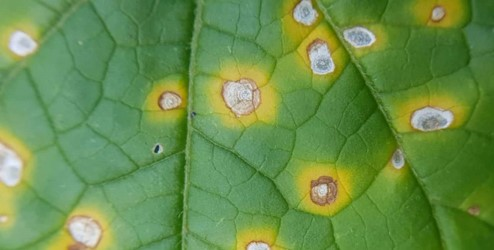
\includegraphics[width=5cm]{spots_on_leaf.jpg} & 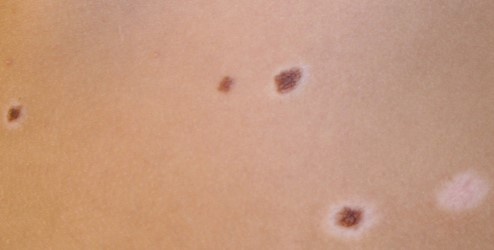
\includegraphics[width=5cm]{sports_on_skin.jpg} \\
    \end{tabular}
}{icon_3.png}

\slidedefault{Introduction}{
    \framesubtitle{Expected results}
    Expected performance order
    \vfill
    \renewcommand{\arraystretch}{1.5}
    \begin{tabular}{l|c|c}\hline
        Pre-training & Plant tasks  & Dermatology tasks \\\hline
        ImageNet (SSL/SL) & \emoji{unicode_1f949.png} & \emoji{unicode_1f949.png}\\\hline
        Plant (SSL/SL) & \emoji{unicode_1f947.png} & \emoji{unicode_1f948.png} \\\hline
        Dermatology (SSL) & \emoji{unicode_1f948.png} & \emoji{unicode_1f947.png}\\\hline
        Random & \emoji{unicode_274c.png} & \emoji{unicode_274c.png} \\\hline
    \end{tabular}
}{icon_4.png}

\section{Method}

\slidedefault{Method}{
    \framesubtitle{Fine-tuning the last layer}
    Standard fine-tuning procedure 
    \begin{itemize}
        \item Last layer as classifier
        \item High computation complexity for all combinations
    \end{itemize}
    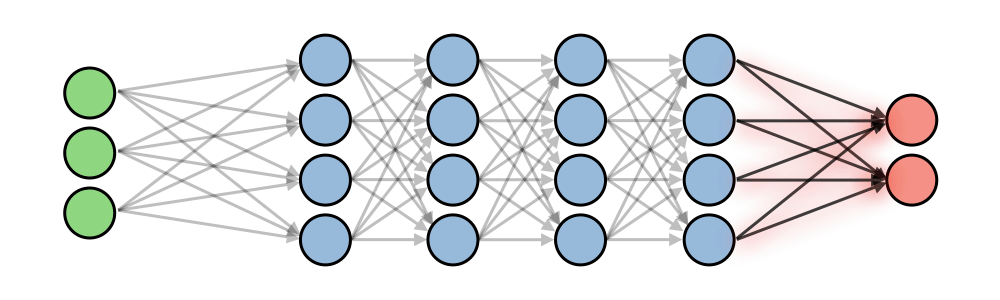
\includegraphics[width=1\textwidth]{fine_tuning_last.png}
    
\includegraphics[width=1\textwidth]{bar_computed.png}
}{icon_11.png}

\slidedefault{Method}{
    \framesubtitle{Frozen evaluation}
    Optimizations
    \begin{itemize}
        \item Fast algorithms like kNN or linear regression
        \item Reusing features
    \end{itemize}
    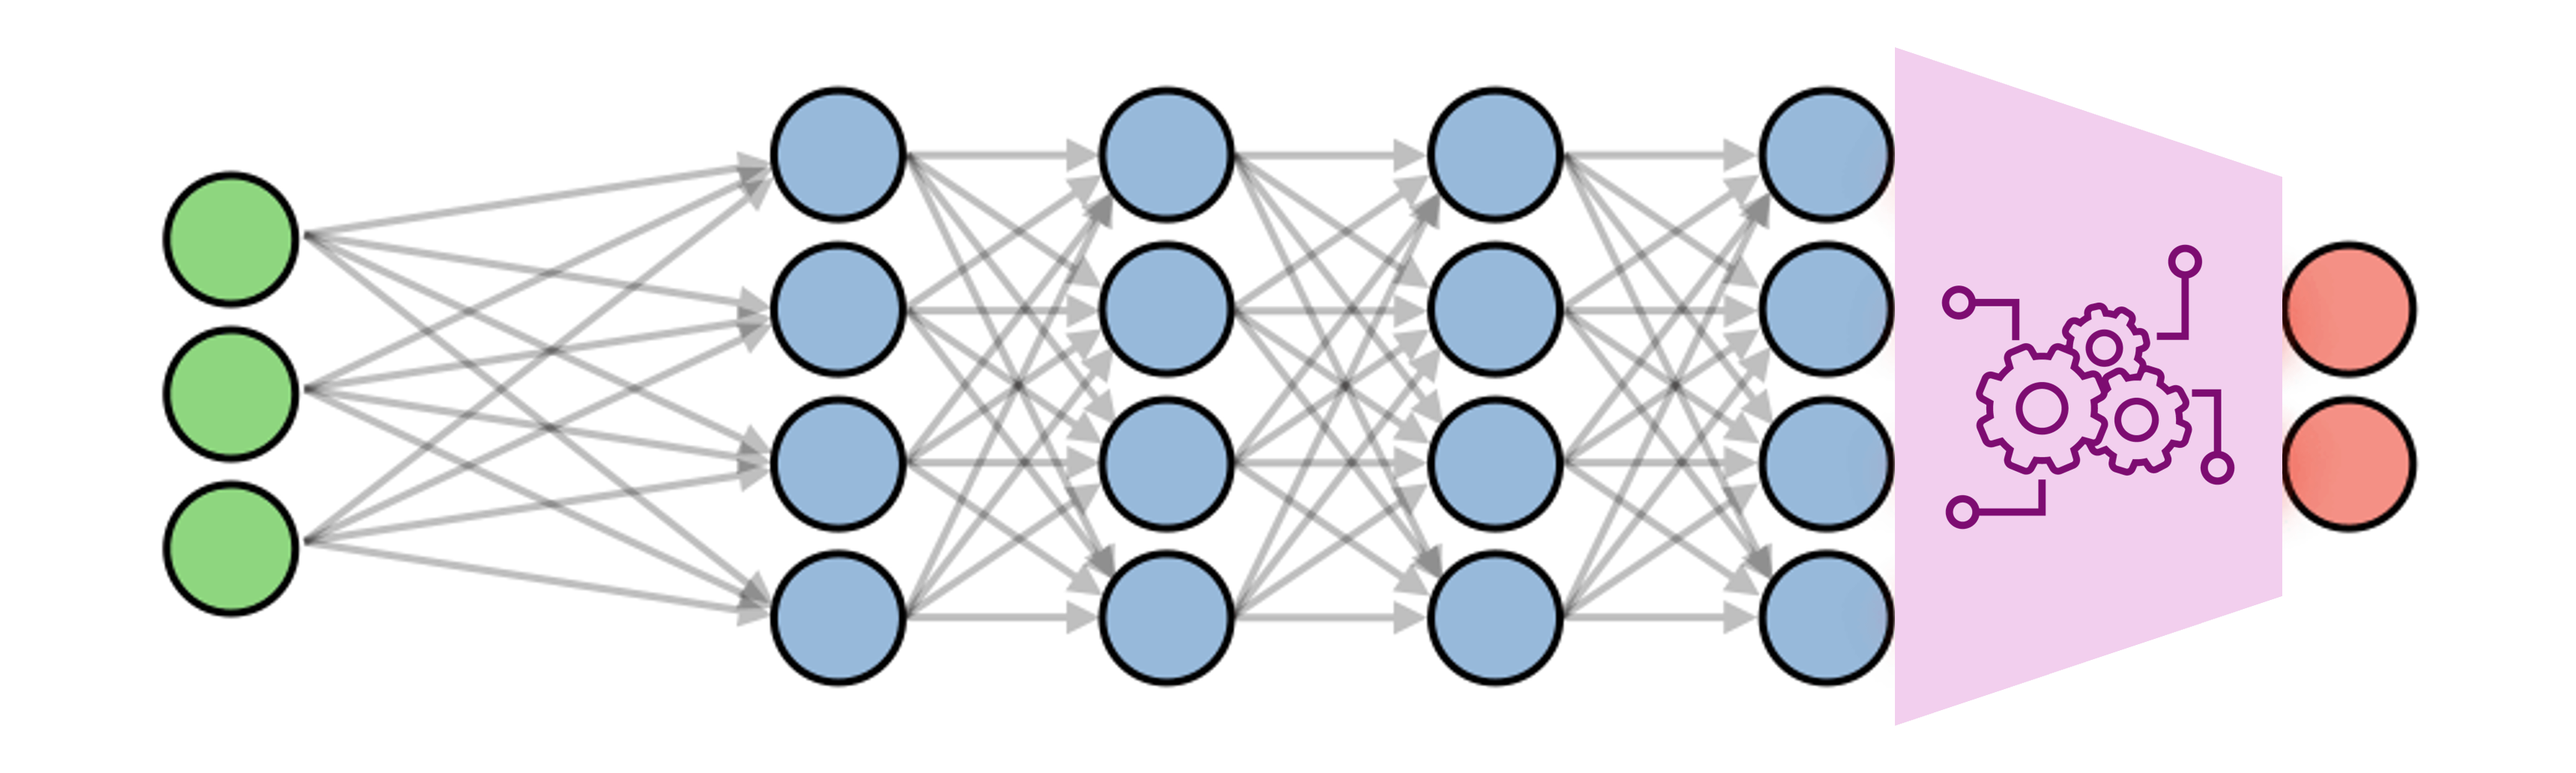
\includegraphics[width=1\textwidth]{frozen_evaluation.png}
    
\includegraphics[width=1\textwidth]{bar_pre_computed.png}
}{icon_13.png}

\slidedefault{Method}{
    \framesubtitle{Datasets}
    \textbf{8 datasets}
    \vfill
    \begin{tabular}{c c c c}
        PlantVillage & Cassava & PlantDataset & PlantDoc \\
        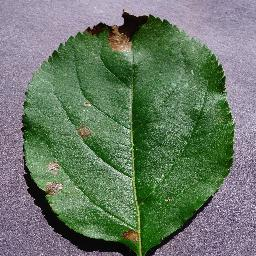
\includegraphics[width=2cm]{sample_plantvillage.jpg} & 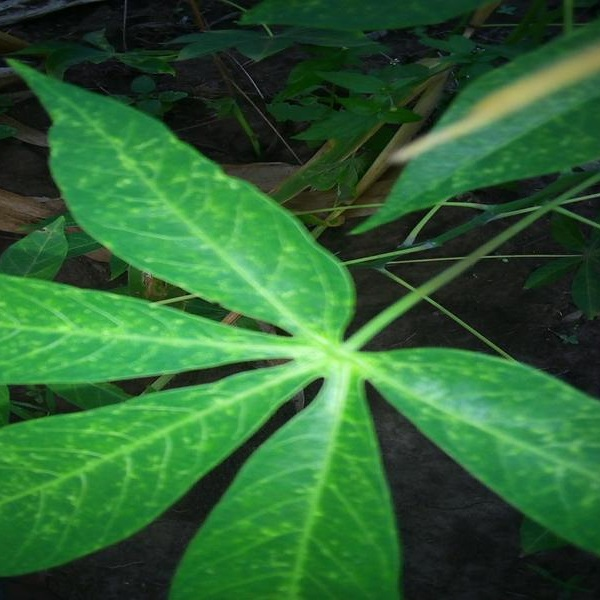
\includegraphics[width=2cm]{sample_cassava.jpg} & 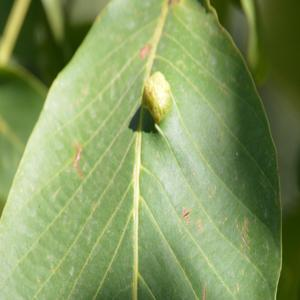
\includegraphics[width=2cm]{sample_plantdataset.jpg} & 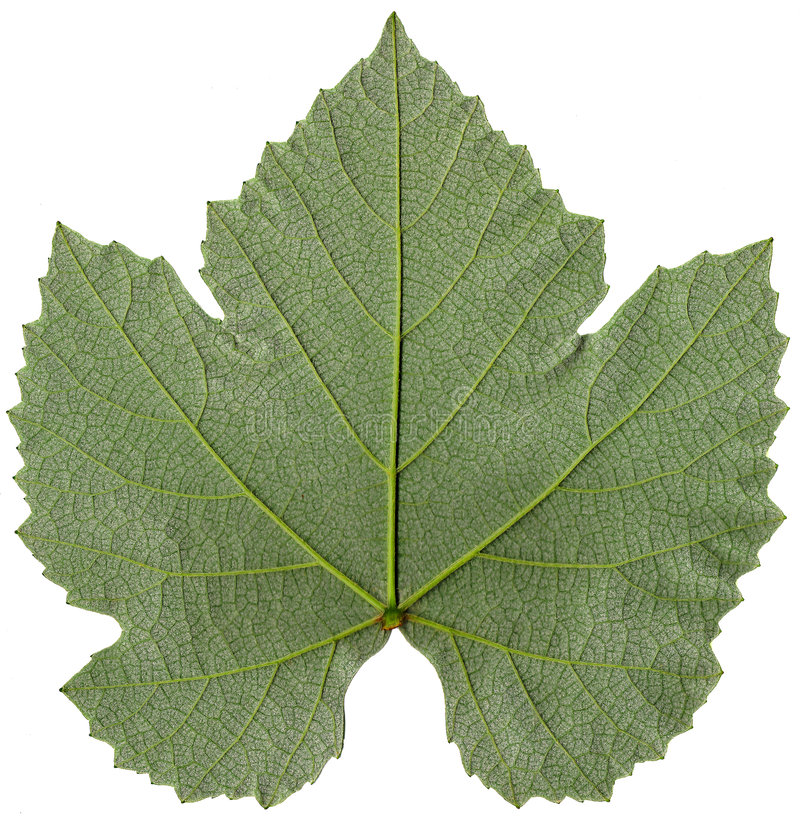
\includegraphics[width=2cm]{sample_plantdoc.jpg} \\
        \\
        DDI & PAD-UFES-20 & HAM10000 & Fitzpatrick17k \\
        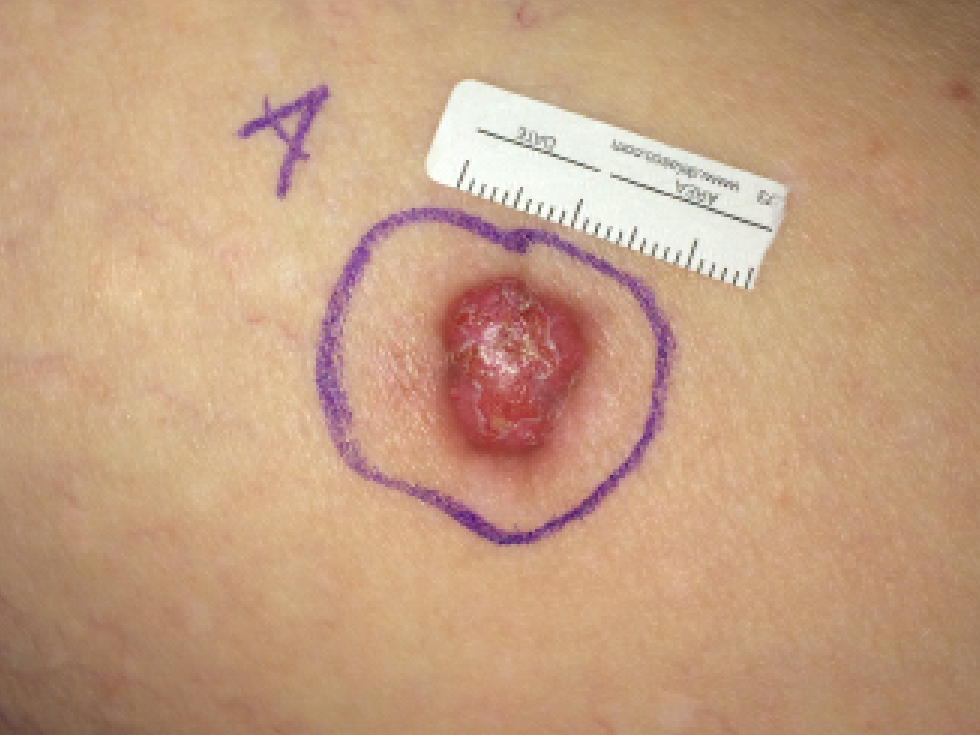
\includegraphics[width=2cm]{sample_ddi.png} & 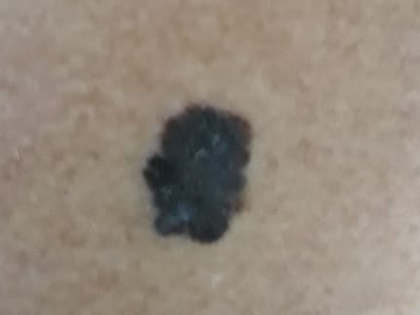
\includegraphics[width=2cm]{sample_padufes20.png} & 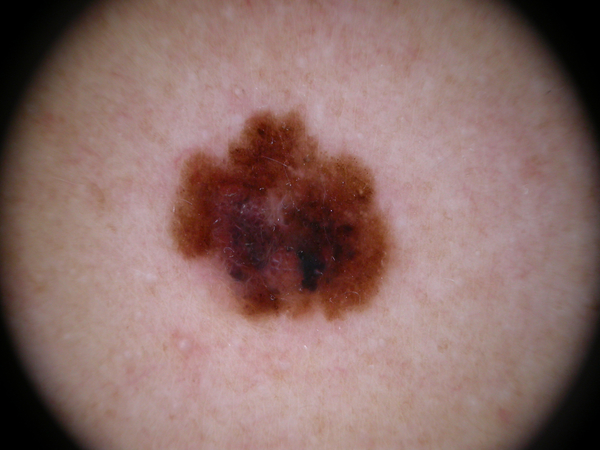
\includegraphics[width=2cm]{sample_ham10000.jpg} & 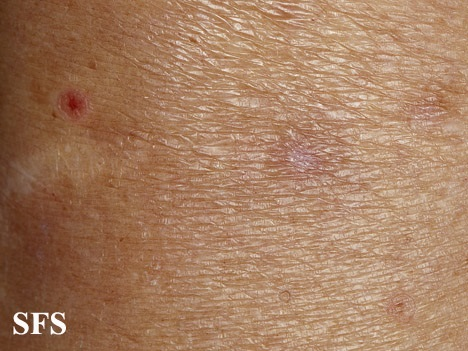
\includegraphics[width=2cm]{sample_fitzpatrick17k.jpg} \\
    \end{tabular}
}{icon_5.png}

\slidedefault{Method}{
    \framesubtitle{Models \& Weights}
    2 architectures with 11 models
    \vfill
    \renewcommand{\arraystretch}{1.3}
    \begin{tabular}{|c|c|c|c|c|}\hline
        \multicolumn{1}{|c|}{} & \multicolumn{2}{c|}{Resnet50} & \multicolumn{2}{c|}{ViT-T/16}\\\hline
        & SL & SSL & SL & SSL \\\hline
        ImageNet & Default & SimCLR & 2x Google & DINO \\\hline
        Dermatology & -- & SimCLR & -- & DINO \\\hline
        Plant & PDDD & -- & -- & DINO \\\hline
        \multicolumn{1}{|c|}{Random} & \multicolumn{2}{c|}{Random} & \multicolumn{2}{c|}{Random}\\\hline
    \end{tabular}
}{icon_7.png}

\section{First analysis}

\slidedefault{First analysis}{
    \framesubtitle{Frozen features}
    Frozen features of PlantVillage visualized with t-SNE
    \begin{itemize}
        \item Structure of similar classes
        \item SL and SSL
    \end{itemize}
    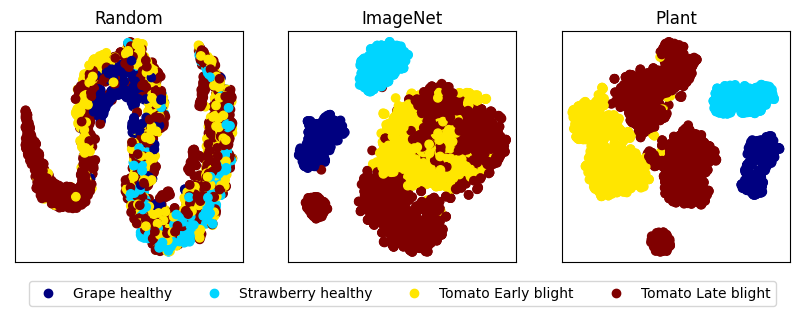
\includegraphics[width=1\textwidth]{features_visualized_with_tsne_combined.png}
}{icon_9.png}

% \textbf{Original} & \textbf{Random} & \textbf{ImageNet} & \textbf{Dermatology} & \textbf{Plant} \\
% 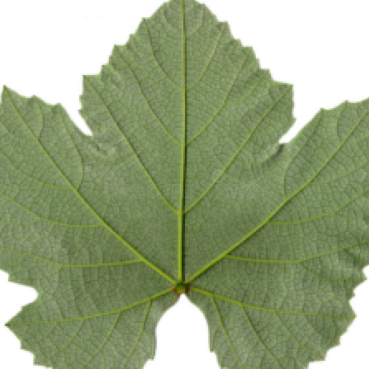
\includegraphics[width=2cm]{attention_input_plantdoc.png} & 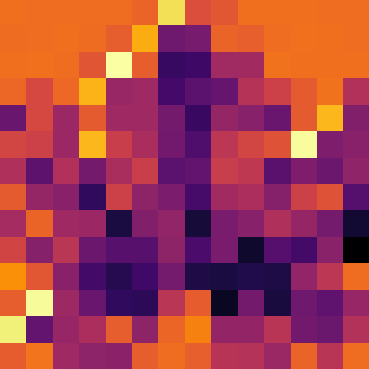
\includegraphics[width=2cm]{attention_ViT_T16-Random_headless_plantdoc.png} & 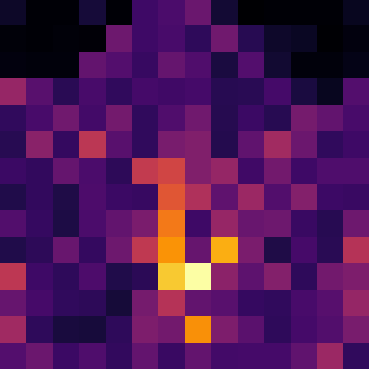
\includegraphics[width=2cm]{attention_ViT_T16-ImageNet_1k_SSL_Dino_headless_plantdoc.png} & 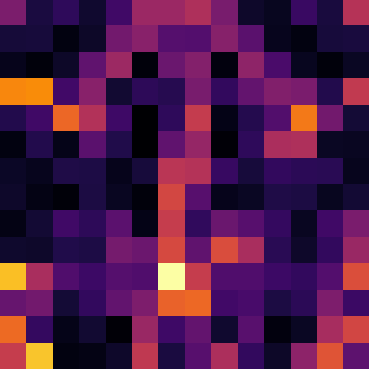
\includegraphics[width=2cm]{attention_ViT_T16-Derma_SSL_Dino_headless_plantdoc.png} & 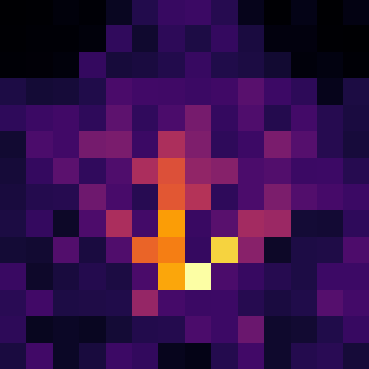
\includegraphics[width=2cm]{attention_ViT_T16-Plant_SSL_Dino_headless_plantdoc.png} \\

\slidedefault{First analysis}{
    \framesubtitle{Model attention random}
    Attention of random model
    \begin{itemize}
        \item Sensitivity to brightness
    \end{itemize}
    \begin{tabular}{c c c c c}
        % \multicolumn{4}{l}{The random model is prone to brightness} \\
        \\
        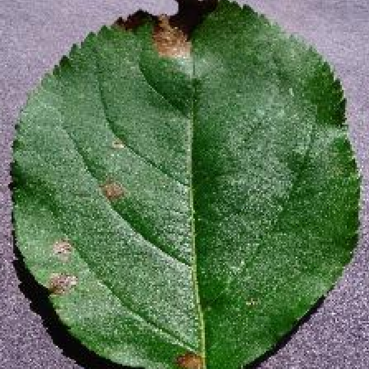
\includegraphics[width=2cm]{attention_input_plantvillage.png} & 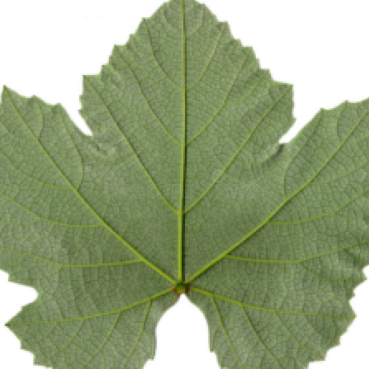
\includegraphics[width=2cm]{attention_input_plantdoc.png} & 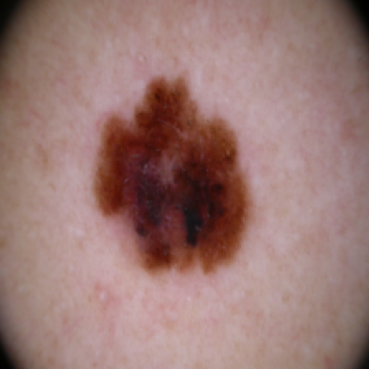
\includegraphics[width=2cm]{attention_input_ham10000.png} & 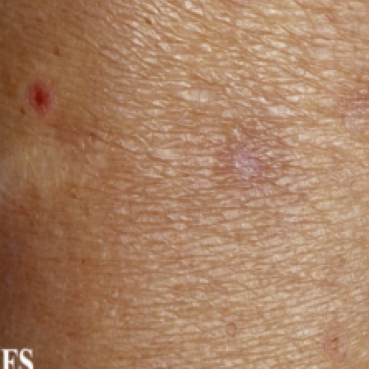
\includegraphics[width=2cm]{attention_input_fitzpatrick17k.png} \\
        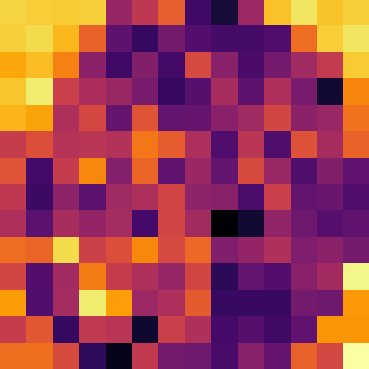
\includegraphics[width=2cm]{attention_ViT_T16-Random_headless_plantvillage.png} & 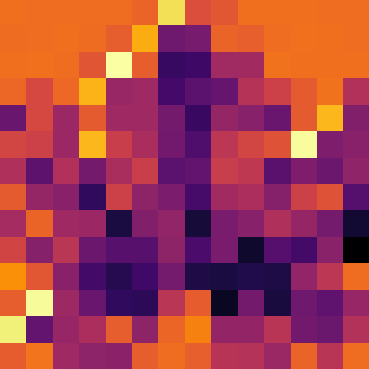
\includegraphics[width=2cm]{attention_ViT_T16-Random_headless_plantdoc.png} & 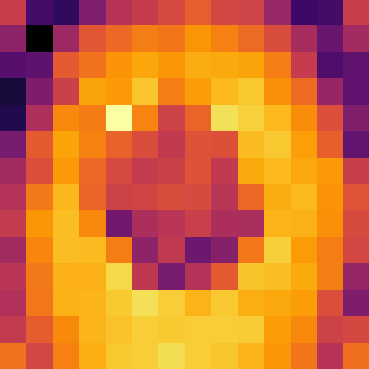
\includegraphics[width=2cm]{attention_ViT_T16-Random_headless_ham10000.png} & 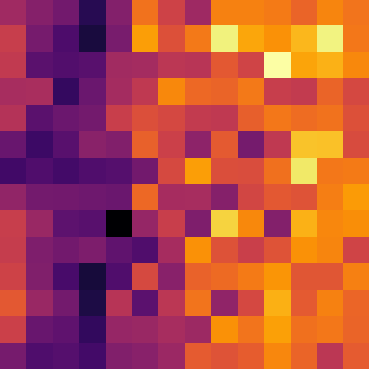
\includegraphics[width=2cm]{attention_ViT_T16-Random_headless_fitzpatrick17k.png} \\
    \end{tabular}
}{icon_8.png}

\slidedefault{First analysis}{
    \framesubtitle{Model attention ImageNet}
    Attention of ImageNet model
    \begin{itemize}
        \item Main focus on abnormalities
    \end{itemize}
    \begin{tabular}{c c c c c}
        % \multicolumn{4}{l}{The ImageNet model mainly focuses on abnormalities} \\
        \\
        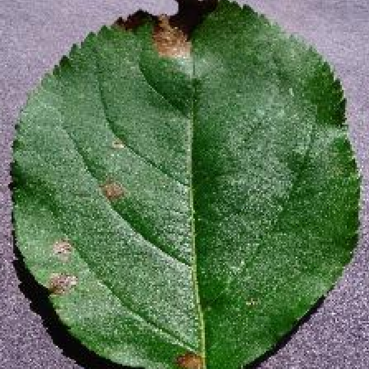
\includegraphics[width=2cm]{attention_input_plantvillage.png} & 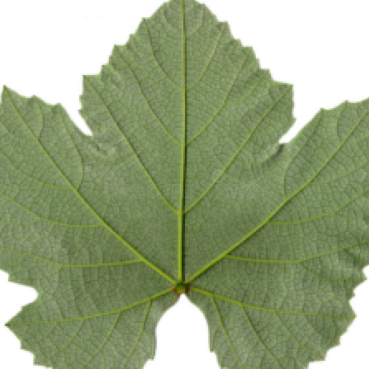
\includegraphics[width=2cm]{attention_input_plantdoc.png} & 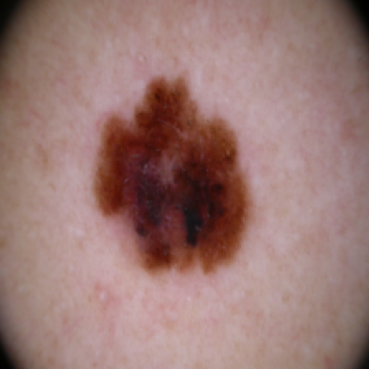
\includegraphics[width=2cm]{attention_input_ham10000.png} & 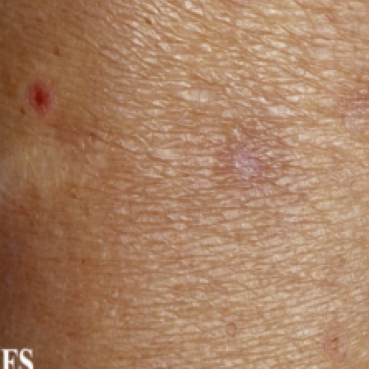
\includegraphics[width=2cm]{attention_input_fitzpatrick17k.png} \\
        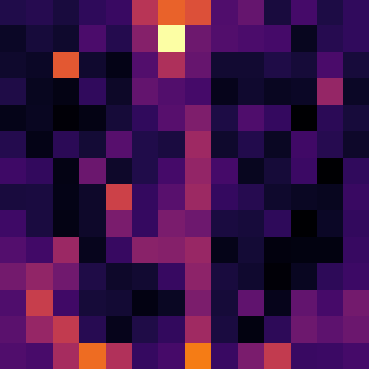
\includegraphics[width=2cm]{attention_ViT_T16-ImageNet_1k_SSL_Dino_headless_plantvillage.png} & 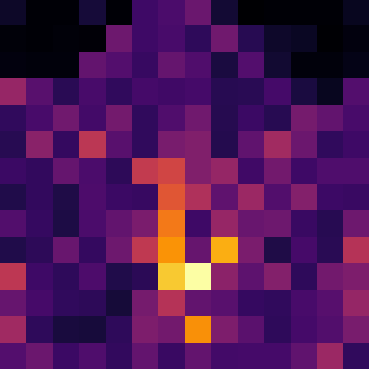
\includegraphics[width=2cm]{attention_ViT_T16-ImageNet_1k_SSL_Dino_headless_plantdoc.png} & 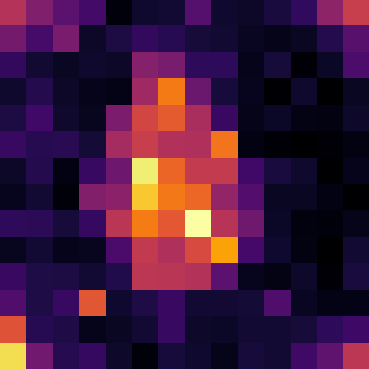
\includegraphics[width=2cm]{attention_ViT_T16-ImageNet_1k_SSL_Dino_headless_ham10000.png} & 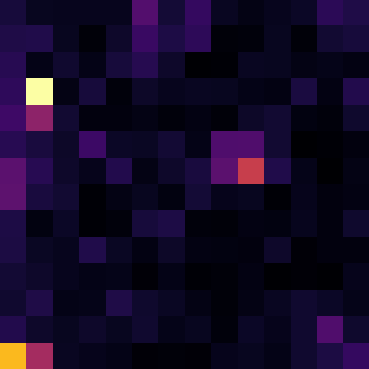
\includegraphics[width=2cm]{attention_ViT_T16-ImageNet_1k_SSL_Dino_headless_fitzpatrick17k.png} \\
    \end{tabular}
}{icon_8.png}

\slidedefault{First analysis}{
    \framesubtitle{Model attention dermatology}
    Attention of dermatology model
    \begin{itemize}
        \item Focus on abnormalities and surrounding area
    \end{itemize}
    \begin{tabular}{c c c c c}
        % \multicolumn{4}{l}{The dermatology model includes the surrounding area} \\
        \\
        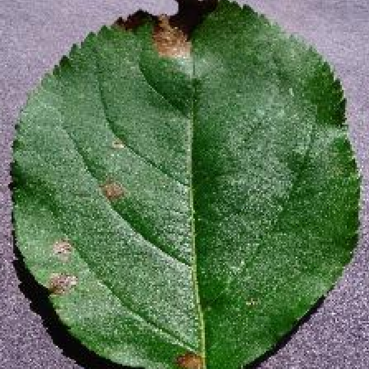
\includegraphics[width=2cm]{attention_input_plantvillage.png} & 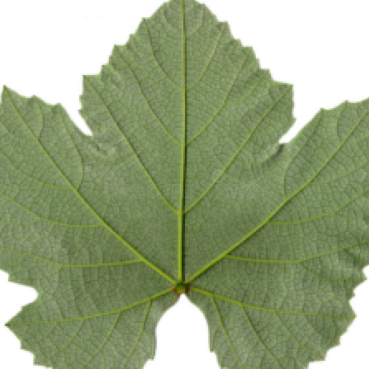
\includegraphics[width=2cm]{attention_input_plantdoc.png} & 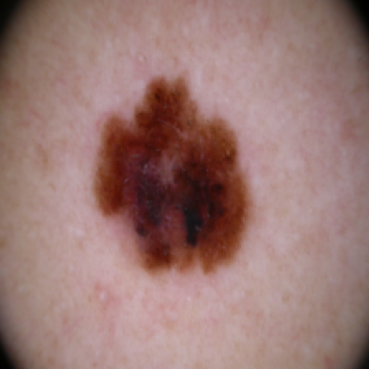
\includegraphics[width=2cm]{attention_input_ham10000.png} & 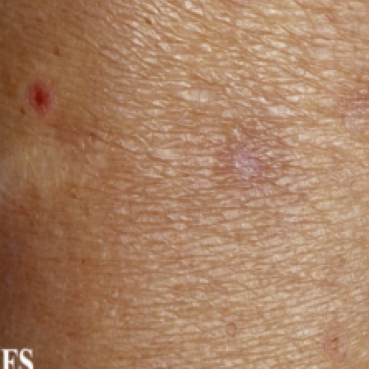
\includegraphics[width=2cm]{attention_input_fitzpatrick17k.png} \\
        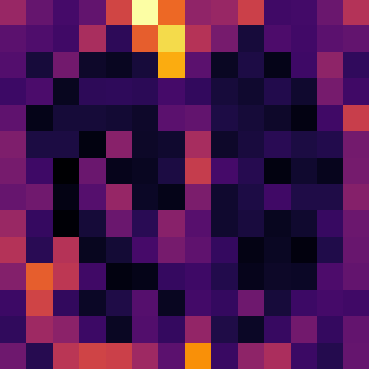
\includegraphics[width=2cm]{attention_ViT_T16-Derma_SSL_Dino_headless_plantvillage.png} & 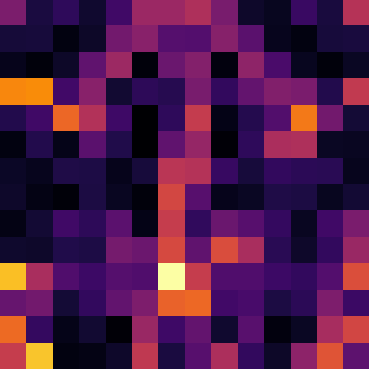
\includegraphics[width=2cm]{attention_ViT_T16-Derma_SSL_Dino_headless_plantdoc.png} & 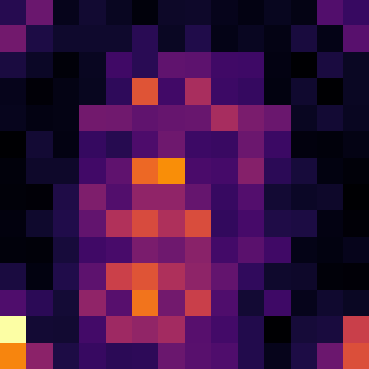
\includegraphics[width=2cm]{attention_ViT_T16-Derma_SSL_Dino_headless_ham10000.png} & 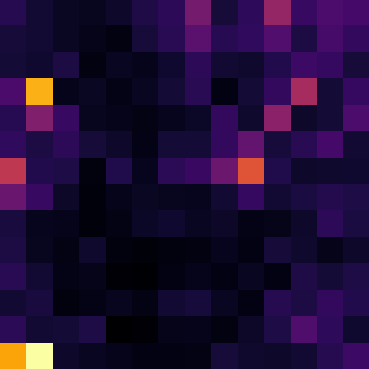
\includegraphics[width=2cm]{attention_ViT_T16-Derma_SSL_Dino_headless_fitzpatrick17k.png} \\
    \end{tabular}
}{icon_8.png}

\slidedefault{First analysis}{
    \framesubtitle{Model attention plant}
    Attention of plant model
    \begin{itemize}
        \item Depiction of the main vein
    \end{itemize}
    \begin{tabular}{c c c c c}
        % \multicolumn{4}{l}{The plant model seems to depict the main vein} \\
        \\
        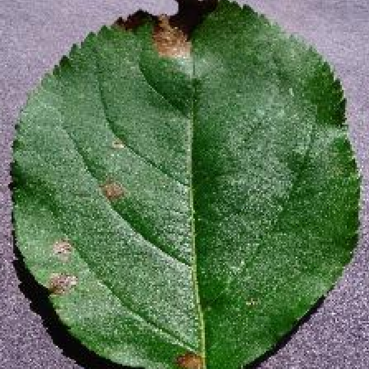
\includegraphics[width=2cm]{attention_input_plantvillage.png} & 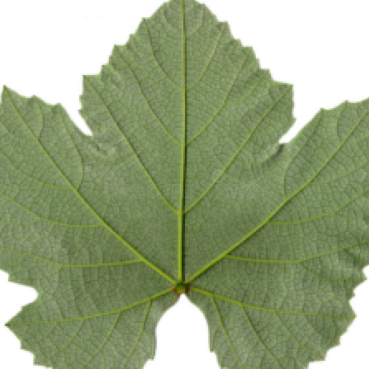
\includegraphics[width=2cm]{attention_input_plantdoc.png} & 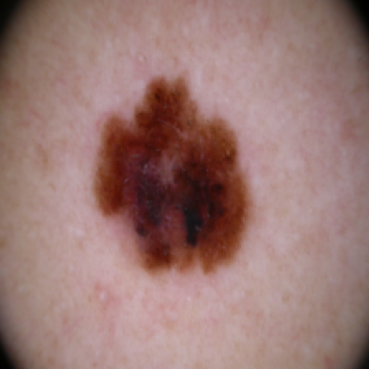
\includegraphics[width=2cm]{attention_input_ham10000.png} & 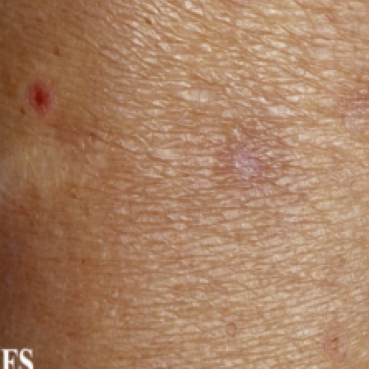
\includegraphics[width=2cm]{attention_input_fitzpatrick17k.png} \\
        \includegraphics[width=2cm]{attention_ViT_T16-Plant_SSL_Dino_headless_plantvillage.png} & \includegraphics[width=2cm]{attention_ViT_T16-Plant_SSL_Dino_headless_plantdoc.png} & \includegraphics[width=2cm]{attention_ViT_T16-Plant_SSL_Dino_headless_ham10000.png} & \includegraphics[width=2cm]{attention_ViT_T16-Plant_SSL_Dino_headless_fitzpatrick17k.png} \\
    \end{tabular}
}{icon_8.png}

\section{Evaluation results}

\slidedefault{Evaluation results}{
    \framesubtitle{Resnet50}
    Average f1-scores from the Resnet50 results
    \begin{itemize}
        \item Bad performance of dermatology
    \end{itemize}
    \includegraphics[width=10cm]{spider_resnet50.png}
}{icon_10.png}

\slidedefault{Evaluation results}{
    \framesubtitle{Vision transformer}
    Average f1-scores from the vision transformer results
    \begin{itemize}
        \item Only one interesting case % add circle
    \end{itemize}
    \includegraphics[width=10cm]{spider_vit_t16.png}
}{icon_10.png}

\section{Subsampling results}

\slidedefault{Subsampling results}{
    \framesubtitle{Overview HAM10000}
    Average f1-scores with limited samples per class
    \begin{itemize}
        \item Expected performance order
    \end{itemize}
    \includegraphics[width=1\textwidth]{lines_ham10000_ViT_T16.png}
}{icon_17.png}

\slidedefault{Subsampling results}{
    \framesubtitle{Training HAM10000}
    Loss curve and f1-score
    \begin{itemize}
        \item Full memorization of training data
        \item Limited generalization
    \end{itemize}
    \includegraphics[width=1\textwidth]{training_ham10000_ViT_T16_Derma_100.png}
}{icon_17.png}

\slidedefault{Subsampling results}{
    \framesubtitle{HAM10000 class comparison}
    confusion matrices of ImageNet and plant model
    \begin{itemize}
        \item Performance of vascular lesions
        \item No obvious connection
    \end{itemize}
    \begin{tabular}{c c}
        \includegraphics[width=4cm]{confusion_matrix_ham10000_ViT_T16_imagenet.png} & \includegraphics[width=4cm]{confusion_matrix_ham10000_ViT_T16_plant.png} \\
    \end{tabular}
}{icon_15.png}

\section{Further experiments}

\slidedefault{Further experiments}{
    \framesubtitle{Fine-tuning multiple layers}
    Fine-tuning vs frozen evaluation
    \begin{itemize}
        \item Multiple layers
        \item Different fine-tuning techniques
    \end{itemize}
    \includegraphics[width=1\textwidth]{fine_tuning_half.png}
}{icon_12.png}

\slidedefault{Further experiments}{
    \framesubtitle{Fine-tuning results}
    
    %TODO matrix
}{icon_16.png}
\section{Discussion}

\slidedefault{Discussion}{
    \framesubtitle{Findings}
    \begin{itemize}
        \item Only one case with expected performance order
        \item Full memorization of training data
        \item Limited generalization
        \item Big differences between Resnet50 and ViT
        \item Attention on text
    \end{itemize}
}{icon_19.png}

\slidedefault{Discussion}{
    \framesubtitle{Further research}
    \begin{itemize}
        \item Data clean up (duplicates, text, false classes)
        \item Comparison of more pre-training algorithms
        \item Standardization of images
        \item Better stopping conditions
    \end{itemize}
}{icon_18.png}

\begin{frame}{Questions and answers}
    \begin{center}
    {\fontsize{40}{50}\selectfont Thank You! \\[10pt] Q \& A}
    \end{center}
\end{frame}

\end{document}
